\chapter{SpaceRL framework}\label{chap:framework}

\newcommand{\toolname}{SpaceRL}

\chapterQuote{\textit{``The introduction of many minds into many fields of learning along a broad spectrum keeps alive questions about the accessibility, if not the unity, of knowledge.''}}{--- Edward H. Levi}

\chapterAbstract{T}{he importance of improving upon the works of others and not just mere replication in scientific reasearch is one of the main pillars of the field. Multiple proposals focus only on publishing their results and not in advancing or even demonstrating the claims the presented in their publications as true, For this reason we present our works as a framework, usable in multiple levels of expertise and meant for expansion. This chapter introduces our framework for KG reasoning and is structured as follows: Section~\ref{sec:framework-intro} Introduces the framework to the reader, Section~\ref{sec:framework-software} described the different components that constitute the framework, Section~\ref{sec:framework-usage} offer an example of use for the framework, Section~\ref{sec:framework-future}describes the possible future for the software, and Section~\ref{sec:framework-summary} closes the proposal.

}


\section{Introduction}\label{sec:framework-intro}

Knowledge graphs (KGs) are sources of structured information that have proved their worth as data structures for the scientific community 
% \cite{SurveyKG} 
and the IT industry alike.
% \cite{noy2019industry}
They provide efficient and versatile support for advanced tasks such as question answering 
% \cite{LiuDXXT22,huang2019} 
or recommendation systems 
% \cite{YangHXL22}
, which is the reason that has led large companies such as Amazon, Google, or Meta, among many others, to use them. 
Information in KGs is generally expressed as a list of facts, which in turn are represented as subject-predicate-object triples made up of two entities and a relation which connects them 
% \cite{schlegel2019}.
 These triples are usually denoted by $\textit(s, r, t)$, which stands for \textit{(source entity, relation, target entity)}. Note that, for the sake of readability, in this paper we use the term \emph{entity} to reference not only an entity itself, but also the node in the graph that contains that entity. 

KGs are usually built from unstructured sources by automated unsupervised processes that extract the information and transform it into triples 
% \cite{paulheim2017, hogan2020}
. However, even the most comprehensive of these processes are always prone to leaving some facts behind, resulting in partially incomplete KGs 
% \cite{BorregoAHRR21}
, which has a negative effect on the performance of the applications that use them.

Several software tools have been proposed to deal with the incompleteness in KGs. Most of them do so by leveraging the information in the graph to infer new triples that represent missing information 
% \cite{chen2020knowledge}
. The approaches in this area can be classified into  four main categories, namely:

\begin{itemize}
    \item Rule-based reasoning 
    % \cite{galarraga2015, kolthoff2015, BorregoAHR019}
    focuses on finding correlations between existing entities in a KG, which when combined with logical operators may infer an existing albeit non-explicit relation between them. This way, the nodes that represent those entities in the graph can be linked, resulting in new triples for the KG. Despite their simplicity, rule-based techniques usually display lower performance than other approaches, since they ignore essential features related to the KG structure.
    
    \item Embedding models 
    % \cite{dai2020survey} 
    transform KG elements into numerical vectors in an N-dimensional space. Embedding-based algorithms then rank the candidate tail entities for a given query \textit{$(s, r, ?)$}, based on their distance to $s$ in the vector space, and retain the top $k$ candidates. The  embeddings generated in this type of algorithms can additionally be used in combination with other techniques (such as Reinforcement Learning), since they provide a compact and informative representation of KG entities and relations. The main drawback of these techniques is that adding new triples to the KG usually entails having to re-compute the embeddings, which is usually a costly procedure.
    
    \item Relation path reasoning 
    % \cite{gardner2015, mazumder2017, BorregoAHRR21}
    focuses on finding paths that indirectly relate two disconnected nodes in a KG. Path-based algorithms build these paths by traversing the graph, and then discern which of those paths actually represent a specific type of relation between the node entities, which is then introduced in the KG as a new triple. The main benefits of these techniques are that they leverage the structure of the KG, resulting in a better performance, and that every path that results in a new triple provides additional explainability for the triple. The main limitation of this type of proposals is that traversing a complete and densely connected web-scale KG can be unfeasible; actually, some of this proposals use a random walk approach, which improves the scalability of the techniques, to the expense of ignoring promising paths in some cases. 
    
    \item Reinforcement Learning (RL) 
    % \cite{xiong2017deeppath}
    path finding enables multi-hop reasoning by using agents to find a path from a source entity to a tail entity that answers a given query.
    The policy-based RL agent learns to traverse the KG travelling from one entity to another adjacent one, and selecting in each step which link to follow, such that this decision maximizes the total episode reward.
    This can be described as a Markov decision process (MDP) which guarantees stochasticity, meaning that the process is non-deterministic. 
\end{itemize}

From the previous analysis, we can conclude that Reinforcement Learning path finding is the most promising approach, since it leverages the KG structure,  provides the same type of explainability as relation path reasoning proposals, while overcoming the scalability problem, and minimizes the risk of neglecting the most promising paths. Furthermore, it can be combined with embedding models to optimize the decision making in each step. Those reasons motivated us to make SpaceRL a RL-based tool for KG reasoning and completion.

There are some previous proposals in this field, such as DeepPath
% \cite{xiong2017deeppath},
MINERVA 
% \cite{das2017go},
Reward Shaping 
% \cite{lin2018multi},
PGPR 
% \cite{xian2019reinforcement},
or DAPath 
% \cite{tiwari2021dapath}.
However, these approaches require the embedding models to be computed beforehand, which hinders their performance. Also, they are restricted to using classical RL algorithms, and overlook the application of more modern RL algorithm such as Proximal Policy Optimization (PPO)
% \cite{schulman2017proximal} 
or Soft Actor Critic (SAC) 
% \cite{haarnoja2018soft}.
Finally, most of these proposals are not distributed as usable tools intended for final users. Even if they make their implementation publicly available, their code is generally intended for the sake of reproducibility of their experimental results, and they often lack any degree of customization or flexibility, meaning they usually can only work on a number of predefined datasets as input.

%Now the benefits, one per 
SpaceRL combines the benefits from RL pathfinding with the power of representational embeddings to infer fairly long and explainable paths, useful for KG-based applications, and it can do so with on-the-fly embedding generation, which means that the KG embeddings are not a required input to the system.

Our tool is highly configurable, allowing for reward calculation to be modified with a combination of several options, customizing the policy intermediate activation function and regularization, using the more classical approach of the REINFORCE .
% \cite{sutton1999policy}
algorithm instead of PPO if required, computing the reward in one of several ways, or selecting the max depth of paths to explore, among other options. Also, SpaceRL allows the user to apply state-of-the-art RL algorithms out of the box, namely Proximal Policy Optimization (PPO)
%  \cite{schulman2017proximal} 
combined with Soft Actor Critic (SAC)
%  \cite{haarnoja2018soft},
which improve performance and help avoid reward plateaus while training. To the best of our knowledge, this is the first tool to provide such a wide variety of options.

Finally, SpaceRL, aims to provide a versatile tool intended for users with different levels of expertise, from novice to experts. It allows comprehensive and flexible customization for advanced users, who may prefer to install SpaceRL as a server for their local usage, or to become a service provider for third parties. On the other hand, it also offers a simple MLaaS interface, intended for a more untrained end user. Machine Learning as a Service (MLaaS) has gained traction in recent years 
% \cite{RibeiroGC15}
, since it adds layers of abstraction that create a black box simplified interface for a non-expert final user. SpaceRL offers RL model generation and usage as a service capabilities, either locally through its GUI or as a deployable REST API for third party consumption. Therefore, it is, to the best of our knowledge, the first turnkey tool to provide such RL KG completion and reasoning functionalities.

\section{Software description}\label{sec:framework-software}
SpaceRL is an end-to-end Knowledge Graph completion tool, written entirely in Python and accessible to multiple user groups with different levels of expertise. SpaceRL provides an easy to use GUI tool for novices, an API for internal network or third party usage, and direct access to the low level application for advanced users or potential contributors. A diagram illustrating its internal code structure is depicted in Figure \ref{fig:classdiagram}.

% \addimage{pseudo_class_diagram.svg}{ SpaceRL package diagram.}{classdiagram}{1} 

\begin{figure}[!h]
    \centering
    \includesvg[inkscapelatex=false, width=\textwidth]{fig/framework/diagrams/pseudo_class_diagram.svg}
    \caption{SpaceRL package diagram.}
    \label{fig:classdiagram}
\end{figure}

SpaceRL was designed to provide a wide variety of functionalities related to KG completion, including: embedding generation, path reasoning model training and testing, integration of pre-trained models, performance metrics calculation and reports, mock KG generation, and cache file generation for distance rewards, among others. Our software includes as well a graphical visualization tool to allow the user inspect the resulting paths inferred from a KG, providing additional information about the reasoning process.

To perform these tasks, SpaceRL requires only a KG as input, which is used to generate different embedding representations of the graph nodes and edges. In its current version, SpaceRL provides support for four classical embedding models in the literature, namely, ComplEx 
% \cite{trouillon2016},
DistMult 
% \cite{yang2015embedding},
TransE \cite{bordes2013translating}, and TransR 
% \cite{lin2015}.
The effectiveness of these models has been confirmed by multiple authors; notwithstanding, further embedding models could be added to SpaceRL in the future. To implement these models, we relied on DGL-KE 
% \cite{zheng2020dgl}
a package which provides off the shelf embedding vector generation.

Our tool is publicly available at our GitHub page 
% \cite{SpaceRL},
and it is open to contribution. The application is divided into several subsystems which will be explored in the following subsections, and the interconnection between these subsystems can be seen in Diagram \ref{fig:tool_flow}. They will be described from the perspective of an advanced user in order to provide a comprehensive view of the proposal.

% \addimage{tool_flow.svg}{SpaceRL work flow}{tool_flow}{.65}

\begin{figure}[htp]
    \centering
    \includesvg[inkscapelatex=false, width=.65\textwidth]{fig/framework/diagrams/tool_flow.svg}
    \caption{SpaceRL work flow}
    \label{fig:tool_flow}
\end{figure}

\lstinputlisting[float, floatplacement=!htp, language=python, label=code:experiment-test-lists, caption=Excerpt of config.py with experimental and testing configuration]{listings/framework/exp_test_declaration.py}

\subsection{Configuration}\label{sec:framework-config} 

The configuration module of SpaceRL comprises two components: a key-value map which holds several global tuning parameters, and the \code{Experiment} and \code{Test} classes. The behaviour of the tool is defined by a list of class instances that describe the experimental and testing setups, respectively, and which can be found in the \code{model/config.py} file (a sample excerpt of this file showing these lists can be found in Listing \ref{code:experiment-test-lists}).

The most relevant global configuration parameters in the key-value map are the following:

\begin{itemize}
 \item \code{activation}  (\code{string}): Indicates what activation function to use in the agent intermediate layer. Available options are: \code{ReLu}
%  \cite{nair2010rectified},
  \code{leaky ReLu}
%  \cite{maas2013rectifier},
  \code{PreLu}
%  \cite{he2015delving},
  \code{eLu}
%   \cite{clevert2015fast},
   or \code{tanh}
%   \cite{lecun1998gradient}.
 \item \code{alpha} (\code{float}): If using Proximal Policy Optimization (PPO), it defines the previous step learning rate.
  \item \code{action\_picking\_policy} (\code{string}): Indicates how actions are selected by the agent in every step of training. Available options are: \code{probability} and \code{max}.
\item \code{episodes} (\code{int}): the number of episodes to train for.
\item \code{gamma} (\code{float}): Decay rate of past observations, used only when \\\code{reward\_type} is set to  \code{retropropagation}.
  \item \code{guided\_reward} (\code{boolean}): If set to \code{false}, a binary reward is used (reward value is either 1 or 0); otherwise, a step-based reward is used, as specified by the \code{guided\_to\_compute} parameter.  
  \item \code{guided\_to\_compute} (\code{list\textless string\textgreater}): If \code{guided\_reward} is set to \code{true}, the user can configure additional options:
  \begin{itemize}
    \item \code{Terminal}: If the agent reaches the target node it overrides other rewards and sets it to 1.
    \item \code{Shaping}: Performs embedding addition of node and relation embeddings to measure the distance from the current node to the target node in vector space.
    \item \code{Distance}: Measures the distance from the agent to the target node.
    \item \code{Embedding}: Combines several vector embedding operations which determine how successful the agent chosen action was towards bringing it closer to the target node.
  \end{itemize}
   \item \code{learning\_rate} (\code{float}): Defines the policy neural network learning rate.
  \item \code{normalize\_embeddings} (\code{boolean}): Normalizes the vector space after performing embedding regeneration.
  \item \code{path\_length} (\code{int}): Specifies  a maximum limit for the inferred paths length.
  \item \code{regenerate\_embeddings} (\code{boolean}): Re-calculates specified embeddings vectors for the desired KG.
  \item \code{regularizers} (\code{list\textless string\textgreater}): Indicates during which training step L1 and L2 regularization should be applied. Available options are: \code{kernel}, \code{bias}, and \code{activity}.
  \item \code{reward\_computation} (\code{string}): Indicates how to calculate the reward value passed on to the learn function to update the policy network based on the agents neural network output. Possible values are:
  \begin{itemize}
    \item \code{max\_percent}: Scales the agent output to [0, 1] where 1 represents the highest output for the step and 0 the lowest.
    \item \code{one\_hot\_max}: Binary reward, 1 for the maximum reward in the episode, 0 otherwise.
    \item \code{straight}: The output from the agent is passed on directly as the reward.
  \end{itemize}
  \item \code{reward\_type} (\code{string}): Indicates how the rewards are propagated to the agent in the learning phase. Available options are: 
 \\ \code{retropropagation} or \code{simple}.
  \item \code{use\_episodes} (\code{boolean}): If set to \code{true}, the agent is trained for the number of episodes specified in the \code{episodes} parameter; otherwise, it relies on the \code{laps} value of the \code{Experiment} class.
   \item \code{use\_LSTM} (\code{boolean}): If set to \code{true}, LSTM layers are added to the agent when generated.
\end{itemize}

Regarding the \code{Experiment} class, it is responsible for agent training, and it requires the following specific configuration parameters: 
\begin{itemize}
    \item \code{experiment\_name(string)}: unique name for each agent.
    \item \code{dataset\_name(string)}: name of the KG used for training.
    \item \code{embeddings(List\textless string\textgreater)}:  embedding model used by the the agent, being the possible options: \code{TransE\_l2}, \code{DistMult}, \code{ComplEx} and \code{TransR}.
    \item \code{laps}: number of laps that are taken by the agent around the KG in order to minimize randomness. Note that larger KGs may require more laps but this increases inference time linearly. 
    \item \code{single\_relation(boolean)}: if \code{true}, the agent trains for a single relation; otherwise, it does so for the entire collection of relations in the KG.
    \item \code{relation(string)}: the name of the relation to train for, if \\\code{single\_relation} is set to \code{true}.
\end{itemize}

The \code{Test} class is tasked with testing the performance of trained agents and generating reasoned paths from this operation, requiring the following parameters:

\begin{itemize}
    \item \code{test\_name(string)}: unique name for each test.
    \item \code{agent\_name(string)}: name that identifies the agent that is going to be tested.
    \item \code{embeddings(List\textless string\textgreater)}: subset of the embeddings used by the agent during training, which will be used for testing.
    \item \code{episodes(int)}: number of tests to perform for the selected agent.
\end{itemize}

\subsection{Reinforcement Learning}\label{sec:framework-reinforcement} 

The RL subsystem takes a KG as an input, and it is responsible for the generation of the training environment, creating the agent that will train on the input KG with the specified configuration options, and managing the data generated during training and testing. 

A Reinforcement Learning \emph{environment} represents the context in which an agent will act and learn. The environment has a \emph{state} that can be manipulated by a number of agent operations called \emph{steps}. However, the agent has only a partial view on the environment in each step,  which puts a limit on the actions it can take; this is referred to as the \emph{action space} available to the agent in the current state. Figure \ref{fig:rl_flow} illustrates how the different Reinforcement Learning modules interact with one another.

% \addimage{RL_Flow.svg}{Reinforcement Learning subsystem work flow}{rl_flow}{1}

\begin{figure}[!h]
    \centering
    \includesvg[inkscapelatex=false, width=1\textwidth]{fig/framework/diagrams/RL_Flow.svg}
    \caption{Reinforcement Learning subsystem work flow}
    \label{fig:rl_flow}
\end{figure}

The subsystem is comprised of a number of classes, namely:  \code{Environment} (\code{model/environment.py}), \code{Agent} (\code{model/agent.py}) and \code{DataManager} \\(\code{model/data/data\_manager.py}). We will explore these classes in depth in the following subsections.

\subsubsection{Environment}

SpaceRL environment is built with navigating the KG in mind; to that effect, we consider that the environment is the entirety of the KG, the state is a particular node in the KG, and the action space is comprised of every relation that links that node with its adjacent nodes (which may include itself).
To create an instance of the environment, a \code{DataManager} class instance is needed, as well as tuning some of the configuration parameters defined in Section \ref{sec:config}: the KG triples, number of laps, and optionally, a specific relation to train for.

The \code{Environment} class was implemented following the OpenAI Gym 
% \cite{OpenAIGym}
standard for reinforcement learning tools, recently transferred to the Farama Foundation and its new drop-in replacement Gymnasium
%   \cite{Gymnasium}.
Enforcing this standard entails the implementation of a number of functions, namely \code{reset}, \code{action\_space}, \code{observation\_space} and \code{step}, with the latter returning the environment state and a \code{done} flag to signal early stopping of the episode. Thus, it is guaranteed that the \code{Environment} class is responsible for state management and action generation. Our implementation also provides on-demand distance cache generation, consultation and reward generation, all of which are used by the agent to drive through the KG.

Once created, the \code{Environment} instance first invokes the \code{KnowledgeGraph} class, initializes the cache, and generates the KG embedding vectors if they are not present, as SpaceRL stores previously generated embedding models while also offering a module to pre-generate them if desired. 

Every training episode begins with a query triple $(s,r,t)$, and the node that contains the head entity $s$ as the initial state of the episode. The selection of the episode initial triple is performed by the environment during the \code{reset} operation. Then, the link representing relation $r$ is then removed from that particular instance of training. Figure \ref{fig:environment} offers a graphical representation of the environment, in which the current state is the initial query triple head entity. 
After the outgoing triple relation is removed, SpaceRL begins the training process. 

% \addimage{env_description.svg}{SpaceRL environment}{environment}{.7}

\begin{figure}[!h]
    \centering
    \includesvg[inkscapelatex=false, width=.7\textwidth]{fig/framework/diagrams/env_description.svg}
    \caption{SpaceRL environment}
    \label{fig:environment}
\end{figure}

For each training step, the environment encodes the initial state as a concatenation of embedding vectors, and calculates all possible actions starting from that state. Then, it relies on the \code{Agent} to select one of those actions in order to advance to the next state. The process is repeated for each state until the episode is complete. In that moment, the reward to be used for policy updates is also calculated based on the configuration parameters chosen.

\subsubsection{Agent}
The \code{Agent} class is one of SpaceRL most complex components, tasked with building the neural network according to a given specification, as well as selecting the actions on each step according to the \code{action\_picking\_policy} and \code{reward\_computation} values in the configuration, memorizing them, storing the rewards given by the environment and advancing to the next environment step.

Creating an instance of the \code{Agent} class requires providing an instance of the \code{Environment} and \code{DataManager} classes, and some configuration parameters, such as the activation function for intermediate layers, the RL algorithm to use, the reward components to activate, and the hyperparameter values \code{alpha} and \code{gamma}.

Once instantiated, the agent initializes its memory and the neural network according to the given configuration parameters. It can do so following a PPO algorithm, which is implemented with an Actor-Critic strategy requiring multiple neural networks, or else by following a classic RL algorithm with a single network.

Subsequently, L1/L2 regularization is configured, the base NN layers are added and then complemented with intermediate LSTM layers 
% \cite{hochreiter1997long}
 if requested. Finally, either ADAM 
%  \cite{kingma2014adam} 
 or RSMprop 
%  \cite{graves2013generating} 
 optimizers are used. If PPO was the selected algorithm, a critic is built sharing its network architecture with the Actor network.

As was described in previous section, class \code{Agent} class intimately interacts with class \code{Environment} during the training episodes. For each action generated by the \code{Environment}, the \code{Agent} calculates the output of the neural network, which represents the score assigned by the agent to that action. Using the scores, the \code{Agent} class evaluates the former actions and selects one of them to proceed, which updates and steps the environment into the next state.
A stopping condition is defined in order to command the agent to end the current training episode. Alternatively, the user may specify a maximum number of steps as stopping condition.  

Machine learning libraries Keras 
% \cite{Keras} 
and Tensorflow
%  \cite{TensorFlow}
are responsible for generating the neural network layered structure and then calculating the outputs on each step and allowing for simple storage and loading of trained models.

\subsubsection{Data Manager}
The \code{DataManager} class is responsible for data storage, modification, and organization during testing, training, and embedding generation processes. 

This class handles KG processing by reading the input KG, expressed as a triple list file and the selected embeddings for training. It then builds two key-value maps, in which the keys are the entities and relations (respectively) for the selected KG and the values are the numerical vectors generated for each chosen embedding. It also handles cached distance rewards, periodically saving the distance cache file, updating it as the training goes on, and improving future agent training.

The \code{DataManager} class also handles persisting and loading agent models, logging information about the training, testing, debugging, and checking the integrity of the system in case an instance of training or testing ended abruptly leaving incoherent files behind.

In summary, the \code{DataManager} class provides the necessary information for other system components (specifically, for the \code{Environment} and \code{Actor} instances) and handles storage of that information in between episodes.

\subsection{Core}\label{sec:framework-core}
The main subsystem of the application acts as the entry point to run a new training or testing process. Its main components are the trainer \code{model/trainer.py} and the tester, \code{model/tester.py}. In the following subsections, they are described in further detail.

\subsubsection{Trainer}
The \code{Trainer} class only requires the configuration key-value map mentioned in section \ref{sec:config} for its initialization. It first detects available GPUs in the system and configures itself to use them if allowed, then instantiates the \code{DataManager}, \code{Environment}, and \code{Agent} classes.
Then, the \code{Trainer} awaits for the \code{run} method to be called, which triggers the training episodes. Each episode starts by obtaining one triple from the Environment, and performing the following actions:

\begin{itemize}
    \item Reset the environment, by setting the state to the head node of the selected triple and removing the outgoing relation from the KG.
    \item Request the \code{Agent} class to select the most promising action to take, along with the reward for the selected action and the maximum reward for the episode.
    \item Advance one step in the environment and update it by taking the action chosen by the agent.
    \item Store the chosen action and its rewards in the agent memory.
\end{itemize}

If the environment activates the \code{done} flag, the episode ends, and the total reward per step is computed and passed onto the agent learning function. Finally, the neural network weights are updated based on the taken path and computed rewards.

\subsubsection{Tester}
The \code{Tester} class needs an already trained agent with which to perform the testing. The \code{Tester} receives the configuration map, the agent model which will be tested, and the embeddings and algorithm that were used during training, as well as the number of training episodes. Then, it performs the setting up operations, namely: configuring the GPU (if available), instantiating the \code{DataManager}, \code{Environment} and \code{Agent} classes, and preparing the models to operate in the environment by replacing the neural network model created for the Agent class with the ones received in the initialization of the \code{Tester} class.

During the testing process, the system iterates through the list of tests in the configuration file (\code{config.py}). For each of them, one agent model and \code{Tester} instance are loaded for each embedding specified in the test configuration. Then, the \code{Tester} executes the specified amount of testing episodes, as described in Algorithm \ref{alg:tester}. 


%explicacion textual del algoritmo
For each episode, the Algorithm tries to infer new paths starting at the head node of the episode triple, and navigating until the maximum the length specified by the configuration parameter (\code{path\_length}) has been reached. Once $10$ paths have been found for the episode, they are ranked based on their scores. Note that we set the limit to $10$ in order to be able to compute the Hits@10 metric value. Finally, the paths that actually reach the episode triple target entity are returned. 

%Comento este párrafo porque según el algoritmo, sí que tiene que haber score
%If necessary, a confidence score is provided that averages the neural network scores for each step of training.

% Hits@N is computed as the number of positive paths (i.e., paths that actually reached the tail entity) that are found within the N first positions of the ranked results, with regard to the total number of triples in the test set. Finally, the average Hits@N value is computed as the average Hits@N values obtained for all the performed tests.

\begin{algorithm}[!h]
    \caption{Testing algorithm}
    \label{alg:tester}

    \KwIn{\\
    $env$: Environment \texttt{// environment instance}\\
    $agent$: Agent \texttt{// pre-trained agent instance}\\
    $config$: Map \texttt{//  configuration key-value map}\\
    $episodes$: Integer \texttt{// total number of episodes}\\
    }
    \KwOut{\\
    $paths$: List\textless path\textgreater \texttt{// map of found paths}\\
    $hits$: Map\textless Int, Int \textgreater \texttt{// map of raw number of hits per N}\\
    $mrr$: Float \texttt{// calculated MRR for agent}\\
    }

    $hits \gets \{1:0$,  $3:0$,  $5:0$,  $10:0\}$\\
    $paths \gets$ [ ] \\
    $ranks \gets$ [ ] \\
    \For{$1$ to $episodes$}{
        $found\_target \gets False$\\
        $local\_paths \gets $ [ ]\\
        
        \For{$1$ to $10$}{
            $triple \gets env.reset()$\\
            $path \gets $[$triple.head()$]\\
            \For{$1$ to $config.path\_length$}{
                $action \gets agent.select\_action()$\\
                $env.step(action)$\\
                $path.add(action)$\\
            }
        $local\_path.add(path, get\_path\_score(path))$\\
        }
        \texttt{// rank paths according to their score}\\
        $local\_paths \gets sort\_paths\_by\_score(local\_paths)$\\
        
        % \texttt{// check for the target entity}\\
        \For{$n, p \gets enumerate(local\_paths)$}{ 
            \uIf{$path\_reached\_target(p)$}{
                $hits \gets add\_to\_hits\_under\_value(hits, n)$\\
                $found\_target \gets True$\\
                $ranks.add(1/n)$ \\
                $break$\\
            }
        }
        \texttt{// if target found, add top path to return list}\\
        \uIf{$found\_target$}{
        $paths.add(p)$
        }
    }

    $mrr \gets ranks.sum()/episodes$ \\
    \Return $paths, hits, mrr$
\end{algorithm}

The evaluation metrics Hits@N and Mean Reciprocal Rank (MRR), are also computed and returned as output of the algorithm (note that we compute Hits@N for N=1, 3, 5, and 10). These are commonly used in the literature to evaluate the performance of ranking algorithms. 
Hits@N results represent the average performance of
the agent over a number of testing episodes. It is calculated by obtaining the 
N first paths in each episode rank, and counting the number of positive episodes, i.e., episodes in which at least one of the N first paths actually reached the target entity. Then, the number of positive episodes is divided between the total number of testing episodes to get the overall Hits@N value for the agent. Function \code{add\_to\_hits\_under\_value} is responsible for this calculation.

MRR is obtained by averaging the rank position value for each path. This value is computed as

\begin{quote}
 \centering
    $ MRR = \frac{1}{N} \sum_{i=1}^{N} \frac{1}{rank_i}$
\end{quote}

where N is the total number of tests, and $rank_i$ is the rank of the top evaluated path that reached the target entity.

The textual representation of the returned paths is stored in a text file in order to be accessible by other processes. 

\subsection{Graphical User Interface} \label{sec:framework-GUI}

SpaceRL offers a GUI that provides the most important functionalities for an average user. The GUI implementation is based on Python default GUI manager Tkinter. An overview of the GUIs elements can be seen in Figure \ref{fig:GUI_structure}.

% \addimage{GUI_view.svg}{ SpaceRL GUI structure}{GUI_structure}{.55}

\begin{figure}[!h]
    \centering
    \includesvg[inkscapelatex=false, width=.55\textwidth]{fig/framework/diagrams/GUI_view.svg}
    \caption{SpaceRL GUI structure}
    \label{fig:GUI_structure}
\end{figure}


When the GUI is launched, the \textbf{main menu} is displayed, as depicted in Figure \ref{fig:mm_default}. The most relevant menu options are the following:

\begin{figure}[!h]
    \centering
    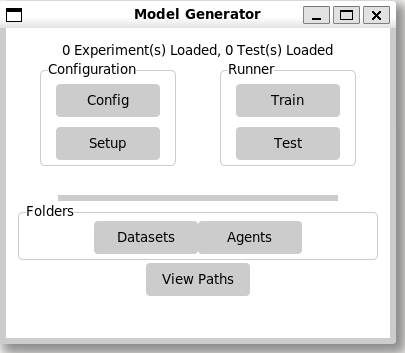
\includegraphics[width=.45\textwidth]{fig/framework/GUI/mm_default}
    \caption{SpaceRL GUI: Main menu window}
    \label{fig:mm_default}
\end{figure}

\begin{itemize}
    \item The \textbf{Configuration} block, which allows the user to open the Config and Setup submenus.
    
    \item The \textbf{Runner} block, which presents the user the options to launch the training and testing processes, respectively.
    
    \item The \textbf{Folders} block, which allows the user to add and remove knowledge graphs. It also includes an option to import pre-trained agent models directly from h5 files, which are native to the Keras environment and preserve all model information.
    
    \item The \textbf{View Paths} option allows the user to generate visualized paths for the tested agents.
\end{itemize}

The \textbf{Config submenu} includes the global configuration parameters described in Section \ref{sec:config}, organized into logical groups. The GUI provides some  descriptive information about these parameters by means of tooltips, which help the user select the most convenient value for each of them. 

\begin{figure*}[!h]
    \centering
    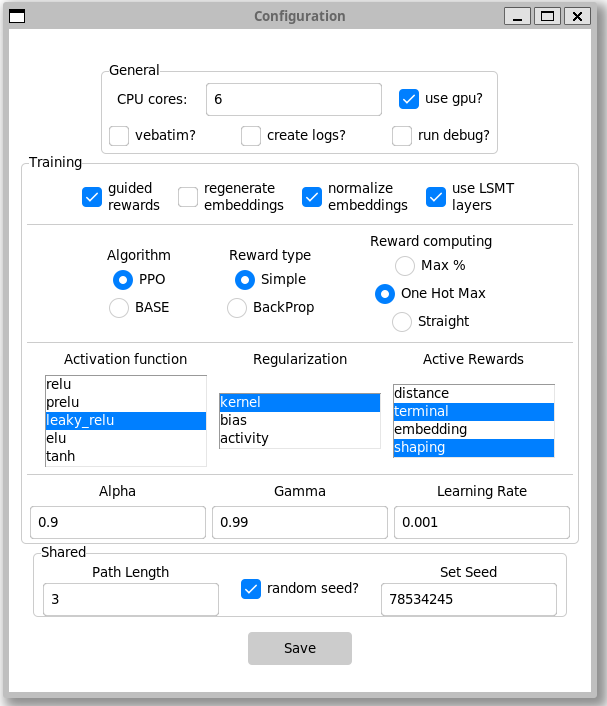
\includegraphics[width=.65\textwidth]{fig/framework/GUI/cm_main}
    \caption{Configuration menu}
    \label{fig:cm_main}
\end{figure*}

\begin{figure*}[!h]
    \centering
    \subfigure[Train submenu presenting 3 distinct experiments listed and an error being displayed]{
        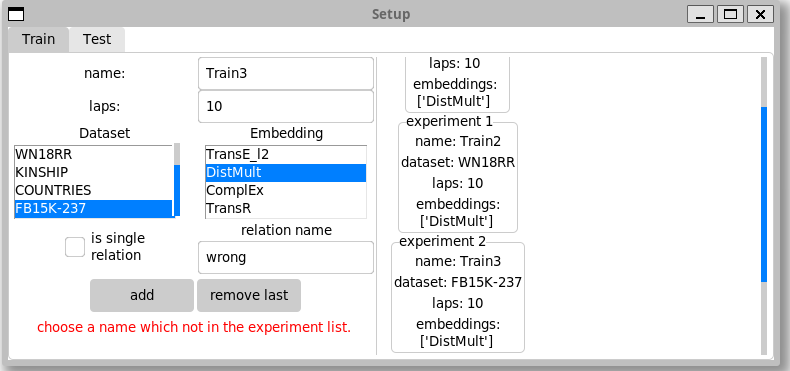
\includegraphics[width=0.65\columnwidth]{fig/framework/GUI/s_queued_train.png}
        \label{fig:s_train_submenu}
    }\\
    \subfigure[Test submenu with several test listed and a suggested embedding for the selected test shown]{
        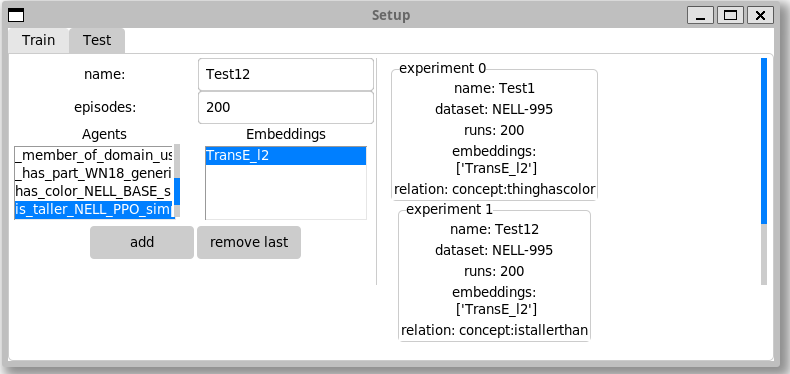
\includegraphics[width=0.65\columnwidth]{fig/framework/GUI/s_queued_tests.png}
        \label{fig:s_test_submenu}
    }\\
    \caption{SpaceRL GUI: Train and test submenus}
    \label{fig:queued_setup_menus}
\end{figure*}

The \textbf{Setup submenu} is divided into two tabs, \textbf{Train} (Figure \ref{fig:s_train_submenu}) and \textbf{Test} (Figure \ref{fig:s_test_submenu}), which include the specific parameters for the training and testing processes, respectively. The tool validates the user input, looking for common mistakes, such as specifying an already existing agent name, an unusually large number of laps, or a relation that does not exist in the given KG. Once the desired experiment or test has been configured, it can be added to the list using the \textbf{add} option at the bottom of each tab. The added elements are then listed at the right side of the corresponding tab, as seen in Figure \ref{fig:queued_setup_menus}.

After the training experiments and tests have been configured, they can be launched using the options available at the \textbf{Runner} block of the main menu (options \textbf{Train} and \textbf{Test}, respectively). The underlying modules are executed asynchronously by means of subprocesses, which enables SpaceRL to run them in the background, and provide real-time progress update through cyclic polling.

\begin{figure*}[!h]
    \centering
    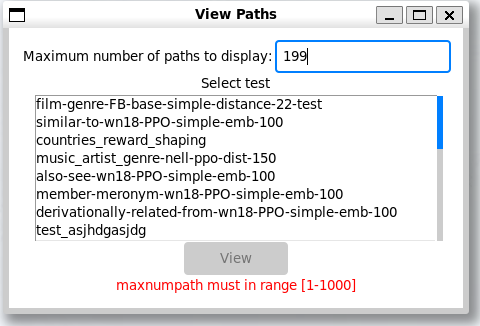
\includegraphics[width=0.47\columnwidth]{fig/framework/GUI/view_paths_menu_error}
    \caption{SpaceRL GUI: Visualization menu}
    \label{fig:view_paths_menu}
\end{figure*}

\subsubsection{Visualizer}
The visualization tool is accessed through the \textbf{View Paths} option in the main menu. First, a window is opened displaying the available test results, to allow the user select one of them. The user also needs to specify the number of paths to load from that test scenario, as seen in Figure~\ref{fig:view_paths_menu} (in the current version, the number of paths is limited to 1000).

After clicking the \textbf{View} button,  the visualization tool main window is opened, displaying one of the paths that led to the target triple and its scores in the selected test, as shown in Figure~\ref{fig:visualizer}. The complete inferred path is displayed at the top of the window in plain text, as the sequence of entities and relations that compose the path. Below, a graph is depicted that illustrates the relevant nodes in the KG, with the available actions at each step. 

Initially, the complete path is shown with only the name of the chosen relations and the score given to them by the agent (step 0). The user can then navigate between path nodes with the arrow keys, thus getting extended information about each subsequent step, namely: the node in which the agent was (highlighted in red), and the score given to each outgoing relation, which corresponds to a possible action that the agent could have taken. The selected actions are highlighted in a bold dark red line. Finally, the arrow buttons on the leftmost and rightmost sides of the screen allow the user to visualize the former and next path, respectively. Note that, in the current version, the paths are displayed to the user in the same order as the agent discovered them.

The implementation of our visualization tool is based on Pygame 
% \cite{PyGame},
which acts as a mediator between SpaceRL and the SDL kit 
%  \cite{SDLKit}
that offers low level access to keyboard, mouse, and graphics hardware. We also relied upon the NetworkX package 
%   \cite{NetworkX},
to compute the 2-dimensional positions of the graph nodes based on the Kamada-kawai distribution 
% \cite{kamada1989algorithm},
and convert these positions into application pixels positions.

\begin{landscape}
    \begin{figure*}[!h]
        \centering
        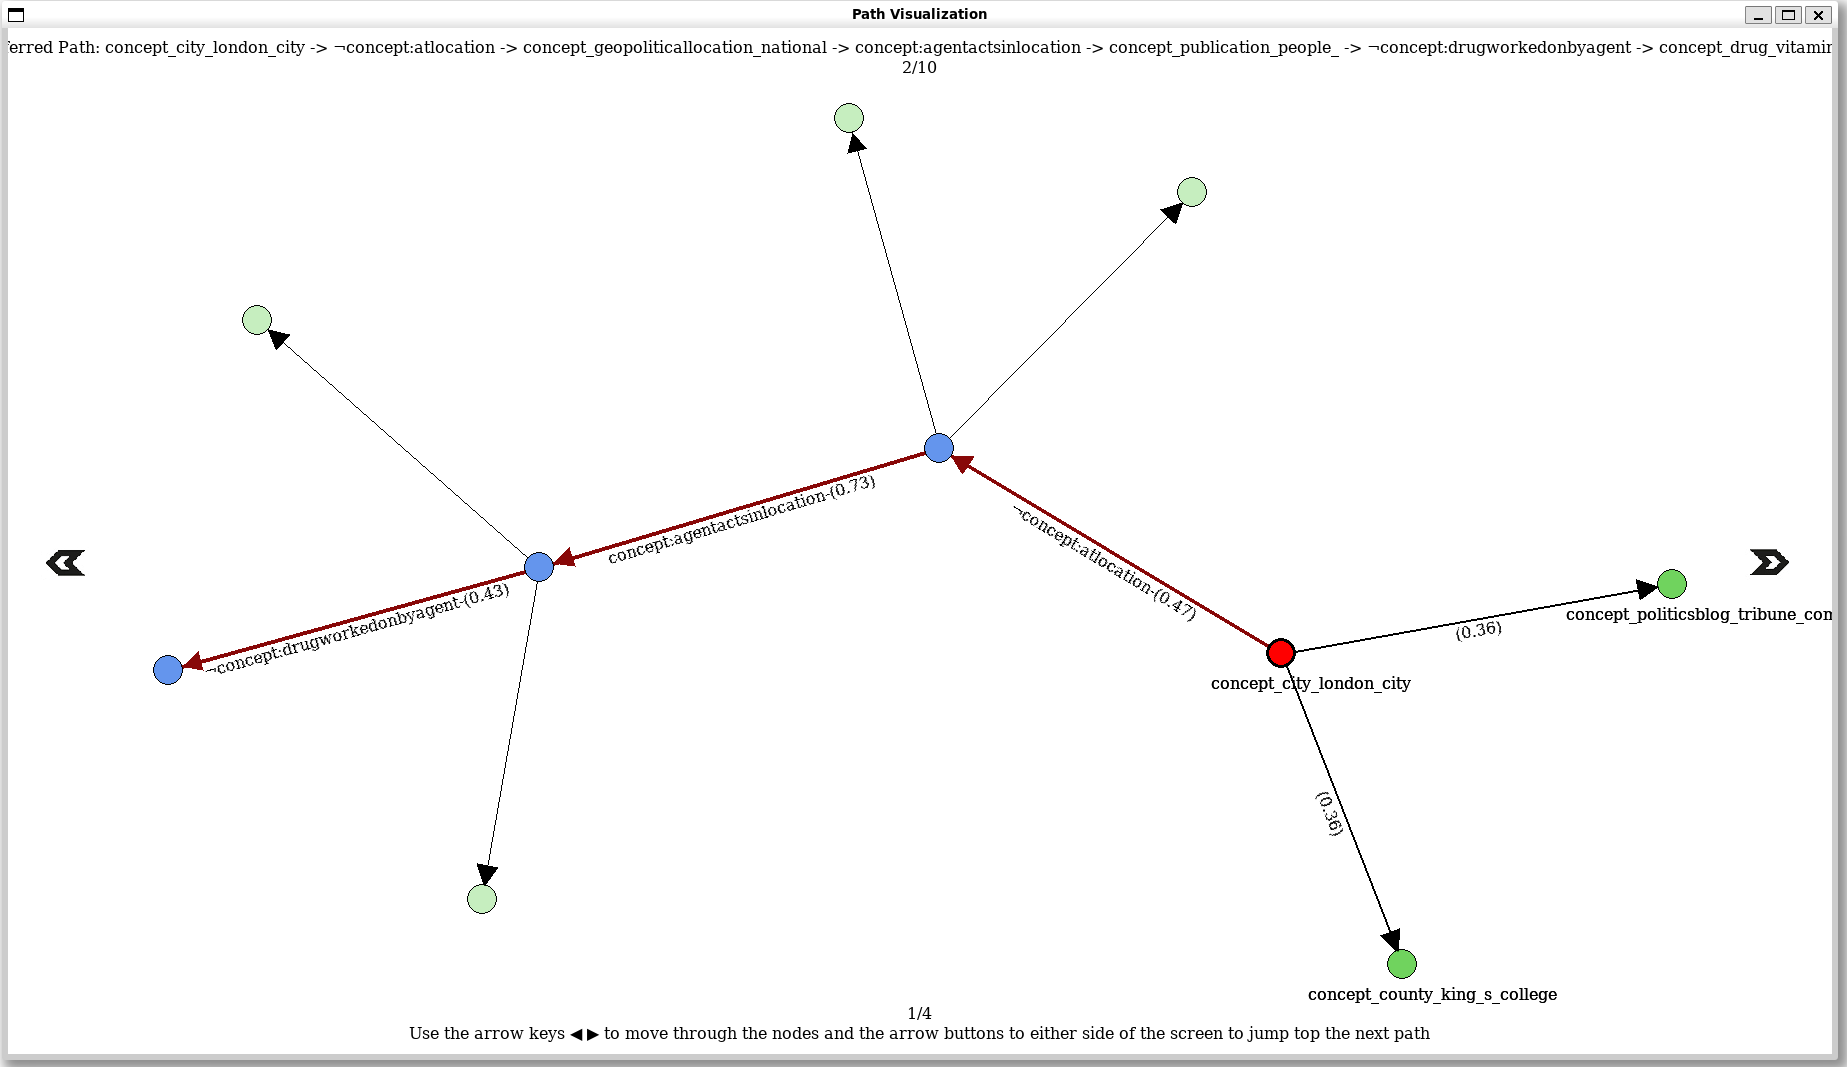
\includegraphics[width=1.65\textwidth]{fig/framework/GUI/Visualizer_2}
        \caption{SpaceRL GUI: Visualization tool.}
        \label{fig:visualizer}
    \end{figure*}
\end{landscape}

%(Figure \ref{fig:API_console}) -> está demasiado lejos la referencia

\subsection{API}
SpaceRL also provides an application programming interface that can be used by developers to implement their own applications on top of our functionalities. Our API service relies on FastAPI
% \cite{FastAPI}
to generate an OpenAPI
% \cite{OpenAPI}
compliant application, and Uvicorn 
% \cite{Uvicorn}
as a backend webserver to host the app. The use of FastAPI makes it easier to deploy it to a production server or to exchange it for another backend if desired.

% API ALLOWS MLAAS COMMENT HERE...

% \addimage{API_view.svg}{API structure of SpaceRL}{API_structure}{0.65}

\begin{figure}[!h]
    \centering
    \includesvg[inkscapelatex=false, width=.65\textwidth]{fig/framework/diagrams/API_view.svg}
    \caption{API structure of SpaceRL}
    \label{fig:API_structure}
\end{figure}

As depicted in Figure \ref{fig:API_structure}, the FastAPI application handles user requests and our \code{ConnectionManager} class holds the internal client-server architecture, which is responsible for resource intensive operations while delivering a response back to the main application to show fast progress to the end user. The \code{ConnectionManager}  class does not rely on intermediate packages to handle requests, which makes it faster and independent from interoperability limitations given by other general purpose software. This, however, adds complexity to the tool, since the implementation of the logic regarding encoding and decoding of requests was custom-made.

FastAPI requires the definition of custom classes to describe the responses returned to the user, as part of the OpenAPI specification. The classes we defined for SpaceRL are the following:

\begin{itemize}
    \item \textbf{Triple} describes entity connection through a given relation.
    \item \textbf{Experiment} describes an experiment suite with a name, the KG to use, the embedding model to use, the number of laps to train, if it is focused on a single relation, and if so, which one.
    \item \textbf{Test} describes a test suite, including a name, the agent name to test, and the number of episodes.
    \item \textbf{EmbGen} is used to generate new embeddings model prior to any experimentation. It is not a necessary step but it makes the training process faster.
    \item \textbf{CacheGen} is used to acquire distance information about a particular KG. It streamlines the training process if distance rewards are used.
\end{itemize}

\begin{figure*}[!h]
    \centering
    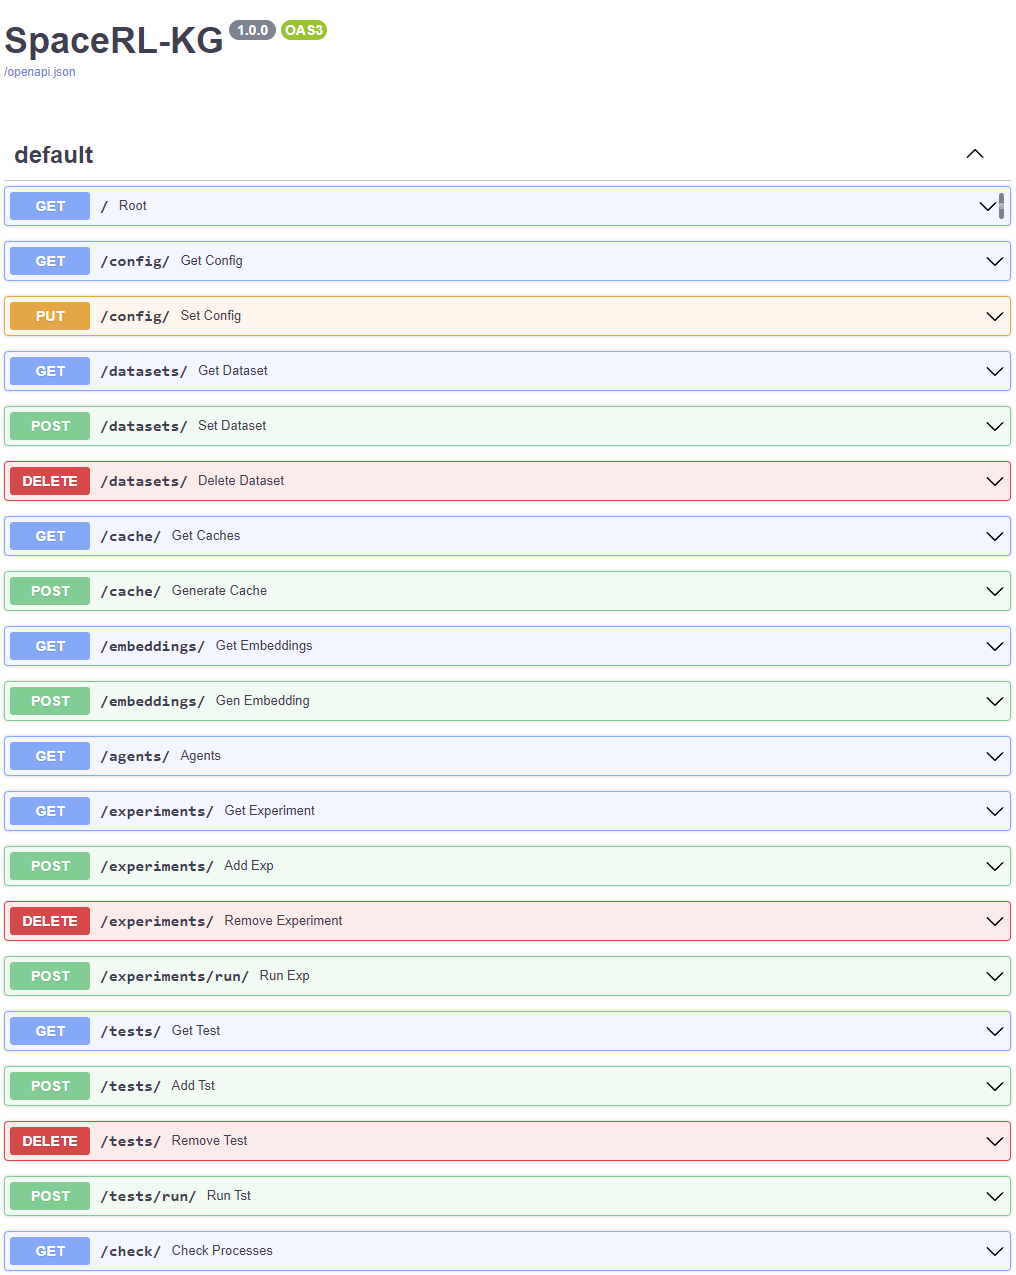
\includegraphics[width=.8\textwidth]{fig/framework/API/api_docs.png}
    \caption{API endpoints}
    \label{fig:endpoints}
\end{figure*}

Figure \ref{fig:endpoints} shows the web view of the API endpoints given by SwaggerUI 
% \cite{Swagger}. 

SpaceRL internally distinguishes  between two types of endpoints, \emph{instant} and \emph{process}. Both provide fast responses to the end user; however, \emph{process} endpoints correspond to computationally intensive background tasks, which require a significant amount of resources. Therefore, the response sent to the user in those cases is merely a message to inform whether the process could be launched. If the resources needed to attend a \emph{process} request are available, the \code{ConnectionManager} underlying client sends a plain-text message to the internal server with the request in a particular format and the server answers back in the same way (cf. listings \ref{code:internal-server-petition-cache} and \ref{code:internal-server-petition-embedding} for examples of these exchanges). 

\lstinputlisting[float, floatplacement=!htp, language=python, label=code:internal-server-petition-cache, caption=Internal server cache generation request and response]{listings/framework/cache_gen_internal.txt}

\lstinputlisting[float, floatplacement=!htp, language=python, label=code:internal-server-petition-embedding, caption=Internal server embedding generation request and response]{listings/framework/embedding_gen_internal.txt}

Next, we provide a description of the available endpoints in detail:

\begin{itemize}
    \item \code{/root} (\emph{instant}): the response is a welcome message as confirmation of a correct deployment, as seen in figure \ref{fig:API_root}.
    
    \item \code{/config} (\emph{instant}): it is used to retrieve (GET) or manipulate (PUT) the configuration key-value map. Only one parameter at a time can be modified, since validation is performed individually.

    \item \code{/datasets} (\emph{instant}): it can be used to get the names of all KGs currently stored (GET), delete existing ones by name (DELETE), or create a new one (POST), by providing a number of triples in the request body.

    \item \code{/cache}: it allows retrieving the name of the KGs that have an associated cache (GET \emph{instant}), and to launch the cache generation process for a specific KG and depth values (POST \emph{process}), by providing a CacheGen instance in the request body. An example request/response for cache generation can be seen in listing \ref{code:internal-server-petition-cache}.
    \item \code{/embedding}: similarly to the cache generation embedding, it also provides a GET endpoint (\emph{instant}) to retrieve embeddings, and a POST endpoint (\emph{process}) that receives a list of EmbGen instances and launches the computation of the corresponding embeddings. An example request/response for  embedding generation can be seen in listing \ref{code:internal-server-petition-embedding}.

    \item \code{/agents} (\emph{instant}): it retrieves all agents stored in the system. The main purpose of this endpoint is to be used together with the testing endpoints (\code{/tests} and \code{/tests/run}).
    \item \code{/experiments} and \code{/tests} (\emph{instant}): They work in a similar way, providing endpoints to insert (POST), retrieve (GET), and delete (DELETE) experiment and testing elements (either individually by id or globally) to the corresponding list. Those elements can then be run by sending a POST request to the corresponding endpoint, either \code{/experiments/run} or \code{/tests/run} (\emph{process}). Optionally, a set of experiment/test ids can be included as parameters in the request body to limit the scope of the training/testing.

    \item \code{/check} (\emph{instant}): it shows the currently active processes on the system, corresponding to elements in the training/testing lists; however, it does not display their current progress. It is used mainly for debugging purposes.
\end{itemize}

Note that SpaceRL accounts for computing resources limitations and it will return a failure message to any request to a process endpoint if it determines that it will cause problems for the host machine. For instance, if there is a embedding generation endpoint running which is using the only available GPU in the system and the \code{/experiments/run} endpoint is invoked with configuration parameter \code{use\_gpu = True}, the API will respond with a \code{BusyError}, notifying the user that there are not enough resources available.

\section{Usages}\label{sec:framework-usage}
adding an example of using the tool such as the one provided in the paper might be usefull to understand how it interact with itself.

The example given must be complete, how to perform it completely with the GUI and how to do it with the API by themselves as standalone applications.


In order to better understand the capabilities of SpaceRL,  we selected NELL
% \cite{mitchell2018}
as an illustrative example. NELL is a knowledge graph with over 50 million triples, which is frequently used as a resource for validation of different proposals for reasoning and completion over KGs.  NELL is built automatically from web data in a continuous and mostly unsupervised fashion, meaning that there are usually a large number of missing triples, which makes it ideal to validate KG completion proposals. For this example, we use a subset of NELL built from the 995th iteration, known as NELL-995
% \cite{xiong2017deeppath}. 

The goal of this section is to use SpaceRL to infer missing links between concepts contained in NELL-995, together with the metric scores associated to the resulting triples, using the capabilities described in section \ref{sec:description}.  We assume that SpaceRL has already been correctly installed, following the instructions available in our GitHub repository 
% \cite{SpaceRL}.

%Más enfasis
We aim to demonstrate the flexibility that SpaceRL provides, which allows to invoke its functionalities either directly, as a local server, or via its API and GUI capabilities, interchangeably. To that effect, we will illustrate how to perform the different steps involved in KG completion using different strategies in each case.

Regarding the API, note that it must be deployed to make its endpoints available. To do so, we must run \code{API/main.py}, and wait for the messages that indicate that both the Internal Server and Client are active, and in which port number is the client application available (cf. Figure \ref{fig:API_console} as an example of these messages).

\begin{figure*}[!ht]
    \centering
    \subfigure[API console]{
        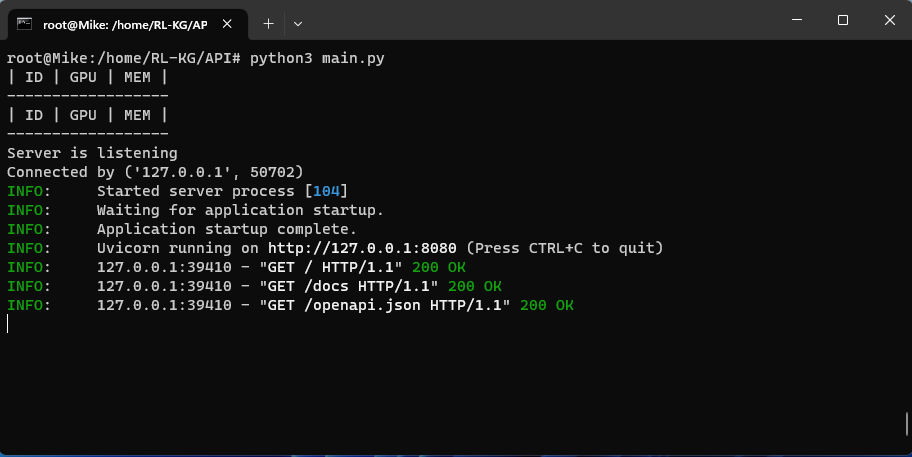
\includegraphics[width=0.43\columnwidth]{fig/framework/API/API_console.png}
        \label{fig:API_console}
    }~
    \subfigure[Default endpoint]{
        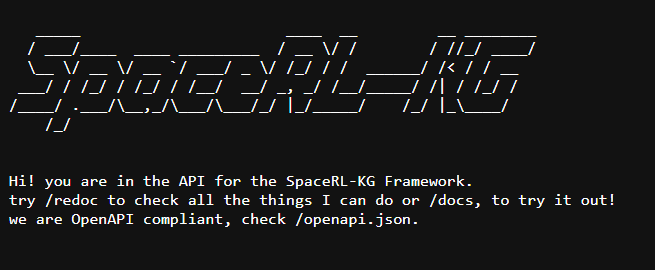
\includegraphics[width=0.51\columnwidth]{fig/framework/API/base_response.png}
        \label{fig:API_root}
    }\\
    \caption{The API being deployed in console and the webserver root}
    \label{fig:API_base}
\end{figure*}

In this example, the API has been deployed to localhost, port number 8080. A request to this address and port will be responded with a welcome message that provides further instructions on how to use the tool, as seen in figure \ref{fig:API_root}. The desired API endpoints are now accessible, which means that any of the existing commercial tools that automatically issue HTTP requests could be used. However, by using FastAPI, SpaceRL is able to provide a web-based, swagger-powered interface in order to access all supported endpoints at url \code{http://localhost:8080/docs}.

As for the GUI, it can be launched by running the file \code{GUI/main.py}, resulting in the main menu windows (cf. Figure \ref{fig:mm_default}).

% PARRAFO DE LO QUE SEA INTEROPERABILITY EQUIVALENT

To perform our sample KG completion, first we must provide the input KG in the expected format, and for this we will directly work on the local instance of SpaceRL. To do so, we create a new subfolder in the \code{/datasets} directory with the desired name,  e.g., ``NELL-995'', and place inside a file named ``graph.txt'' that contains the list of triples that compose the KG. The expected file format is illustrated in listing \ref{code:dataset-base-format}, i.e., one $(s,r,t)$ triple per line, being each triple a sequence of three tab-separated values ($s$, $r$, and $t$). Note that this process could be performed as well using the API (endpoint \code{/dataset}), or the GUI (option \textbf{Datasets} in block \textbf{Folders})

\lstinputlisting[float, floatplacement=!htp, language=python, label=code:dataset-base-format, caption=An extract of NELL dataset with the expected format.]{listings/framework/dataset_format.txt}

Then, we need to provide the desired configuration for SpaceRL, including the global parameters, and the specific training and testing parameters, as described in Section \ref{sec:config}. The values for the configuration key-value map parameters can either be set using the \textbf{Config submenu} (cf. Figure \ref{fig:cm_main}), the \code{/config} API endpoint, or directly by editing the configuration file \code{/config.py}, as shown in listing \ref{code:configuration-file}, which also displays other possible values that the parameters can take as Python-style comments.

\lstinputlisting[float, floatplacement=!htp, language=python, label=code:configuration-file, caption=Configuration parameters used for the example]{listings/framework/config.py}

The next step is embedding generation, which could be omitted, since SpaceRL is able to perform it automatically. In this case, however, in order to further illustrate these functionalities in detail, all embedding representations for the NELL-995 KG will be generated. To do so, we can issue an HTTP POST request to endpoint \code{/embeddings}, including in the request body the parameters shown in listing \ref{code:embedding-request}.

\lstinputlisting[float, floatplacement=!htp, language=json, label=code:embedding-request, caption=The request body parameters to generate all embeddings for NELL KG.]{listings/framework/embedding_req.json}

This request will trigger the internal client to communicate with the server and initiate the embedding generation. Then, a response is sent to the API client with information regarding whether the operation has began correctly, or if any error has occurred, e.g., if the server resources are busy and the request cannot be attended. 
Meanwhile, the application console displays the internal client-server communication messages, as seen in Listing \ref{code:internal-embedding-request}.

\lstinputlisting[float, floatplacement=!htp, language=json, label=code:internal-embedding-request, caption=Internal client-server communication for embedding generation request.]{listings/framework/embedding_gen_internal.txt}

As a result, new files are added to folder \code{datasets/NELL-995}, namely \code{entities.tsv} and \code{relations.tsv}, which hold all entities and relations of the KG, respectively, with an assigned id. Also, a new \code{/embedding} subfolder is created, which holds the results of the embedding vector generation operation performed by DGL-KE for each of the required models (ComplEx, 
 DistMult, TransE, and TransR,  in the current version).

Finally, to generate the RL agents, new experiments must be added to the experiments list, via HTTP POST requests to the \code{/experiment} endpoint, providing the necessary parameter values in the request body. An example of a new experiment that uses TransE embeddings and 150 laps to train on the  NELL-995 KG can be seen in Figure \ref{code:train-request}.

\lstinputlisting[float, floatplacement=!htp, language=json, label=code:train-request, caption=The request body parameters to generate a NELL RL Agent]{listings/framework/exp_req.json}

In response to the former request, the server responds with an informative message (e.g., in case of success, the message returned is:
\\
\\
``\code{Success}'': ``\code{experiment successfully added to queue.}'').
\\
\\
Some other operations that could be performed at this point are: checking the state of the queue through the same \code{/experiment} endpoint using a GET request, deleting queued elements through the DELETE request in the same endpoint, or adding more experiments to the queue by repeating the process above. For instance, if we wanted one agent for each of the embedding models we could repeat the process above to create 4 queued experiments, one per supported model.

Then, the experiments would be run by issuing a POST request to the \code{/experiment/run} endpoint, which expects a list of ids to run, or an empty list, in  which case all queued experiments are run. Again, the API responds with and informative message (e.g., in case the operation was successful, the message would be :
\\
\\
``\code{Success}'':``\code{Experiment(s) Launched}'').
\\
\\
The agent generation operations can be computationally complex, which is why SpaceRL provides two mechanisms to track their progress:
\begin{itemize}
    \item \textbf{Log files}, which are redirected console output from the server which is running the process, found as \code{logs/p\_ExperimentRunner.out} and \code{logs/p\_ExperimentRunner.err} for the general and error outputs, respectively.
    
    \item The \code{/Check/} debug endpoint,retrieves a list of active processes in the application console, named according to the task they perform. In our example, a request to this endpoint yields the following response:
    \\
    \\
    ``\code{Success;[\textless name=`ExperimentRunner', [...], started\textgreater]}''

\end{itemize}

Once the operation is complete, a new folder is created at \code{model/agents/\\My\_New\_NELL\_Agent}, which contains the configuration options used to generate the agent, and the models that comprise it.
The generated agent can be used as input to a testing process, to assess its performance and use it to infer new paths for NELL-995.

As we stated before, all the former operations could have also been invoked via our GUI. For the remainder of this Section, we will focus on this part of SpaceRL, although the testing functionality could also be invoked via the API.

Once the main GUI window is displayed, the \textbf{Config} option under the Configuration block opens the configuration submenu window (Figure \ref{fig:cm_main}). This window reflects the changes made to the key-value map in the \code{config.py} file, and allows for further tuning. 

To proceed with testing we choose the \textbf{Setup} option under the Configuration block, which opens the training and testing submenu (Figure \ref{fig:s_NELL_test}). In this example, we select the Test tab, in which the generated agent can be picked out from a scrollable select input.

When an agent is selected, the available embeddings are displayed in another select input next to the first one. Additionally, we need to provide a name for the Test instance and a number of test episodes, and then click on the \textbf{add} option. The right side of the window displays the list of available tests to be run. 

\begin{figure*}[!ht]
    \centering
    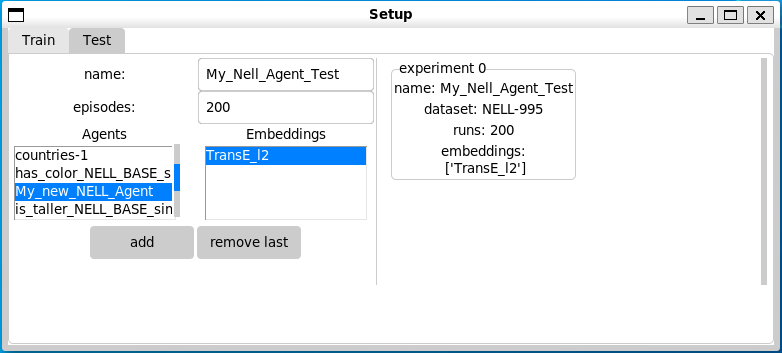
\includegraphics[width=.75\textwidth]{fig/framework/GUI/NELL_agent_test.PNG}
    \caption{Testing submenu with NELL Agent being tested.}
    \label{fig:s_NELL_test}
\end{figure*}

Back to the main menu window, we can use the \textbf{Test} option in the Runner block to launch as many instances of the \code{Trainer} class as needed,  and perform up to 10,000 tests at a time for each of the elements in the test list.

\begin{figure*}[!ht]
    \centering
    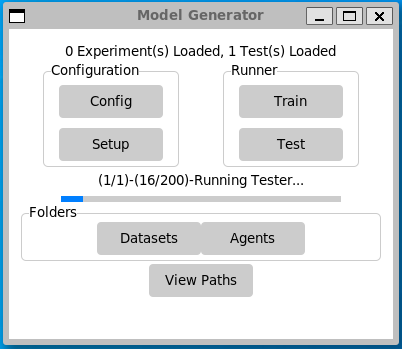
\includegraphics[width=.5\textwidth]{fig/framework/GUI/NELL_agent_running.PNG}
    \caption{Main menu with running test}
    \label{fig:mm_NELL_test}
\end{figure*}

The main menu (Cf. Figure \ref{fig:mm_NELL_test}), now displays the progress of the current operations. Note that in the text above the progress bar, ``(1/1)'' indicates that only 1 element is queued for testing while ``(16/200)'' expresses the current and total episodes being run.

Once the execution is finished, a new folder is created in \code{model/data\\/results/My\_NELL\_Agent\_Test}, containing a \code{metrics.csv} file with the Hits@ and MRR metric values, and a \code{paths.txt} file containing the inferred paths in this testing execution. Examples of the resulting metrics and the inferred new paths can be found in Listings \ref{code:metrics} and \ref{code:path}, respectively.

\lstinputlisting[float, floatplacement=!htp, language=XML, label=code:metrics, caption=The metrics obtained from testing the Nell-995 agents for 200 episodes.]{listings/framework/metrics.csv}

\begin{table}[!h]
    \centering
    \begin{tabular}{l|l|l}
    \hline
        \multicolumn{3}{c}{NELL-995} \\ \hline
        hits@1 & TransE\_l2 & 0.565 \\ \hline
        hits@3 & TransE\_l2 & 0.755 \\ \hline
        hits@5 & TransE\_l2 & 0.95 \\ \hline
        hits@10 & TransE\_l2 & 0.99 \\ \hline
        MRR & TransE\_l2 & 0.6723 \\ \hline
    \end{tabular}
    \caption{Metrics obtained from testing the Nell-995 agents for 200 episodes.}
    \label{tab:metrics}
\end{table}


\lstinputlisting[float, floatplacement=!htp, language=python, mathescape=true, label=code:path, caption=An example of a returned path by the agent.]{listings/framework/paths.txt}

Observing the previously mentioned listing we can see how a typical evaluation result  would appear, the first column indicates the metric that was evaluated, the second column specifies which embedding model was used, and finally, the third column displays the value of said metric. In the provided example, there is only one row for each metric, since only one embedding model (TransE) was tested.

On the other hand, in listing \ref{code:path} we can see an example of a newly reasoned path. The path is expressed as the alternating sequence of entities and relations that must be traversed to get from the source entity until the target entity. This path provides some explainability regarding the existence of the initial query triple. For this particular example, we would have the following logic:

\begin{itemize}
    \item Alan Greenspan is a top member of the US federal reserve.
    \item Ben Bernake is also a top member for the US federal reserve.
    \item Ben Bernake works for the federal reserve.
    \item Therefore, Alan Greenspan also works for the federal reserve.
    \item As a consequence, fact ``(concept\_ceo\_alan\_greenspan, concept:worksfor,\\  concept\_bank\_federal\_reserve)'' should be added to the KG.
\end{itemize}

\section{Support and Iterations}{sec:framework-future}
% the future of the tool, possible limtations and changes

SpaceRL is Open Source software, open for collaboration in its GitHub repository \cite{SpaceRL} and being improved constantly. Therefore, not only does it provide benefits for companies whose business model is based on knowledge graphs and need to manipulate them; it could also be potentially benefitial for researchers in data engineering areas who can use our functionalities as a solid support to build their own smart applications.

Finally, our tool could also aid researchers in other areas, such as biomedicine, statistics, or data science, who do not possess a computing science background that allows them to build their own software, but still require this kind of tool to operate on their knowledge graphs.


We made sure that, as Open Software, SpaceRL is easily expandable by keeping the dependencies to a minimum whenever possible, providing extensive documentation and following community standards such as OpenAPI and Gymnasium.

The future steps in the life cycle of SpaceRL would be to design modular reward and policy elements which could be altered by experts to increase its reach even more, to offer a large scale implementation to support uncoupled operations and to increase the level of the documentation offered

\section{Summary}\label{sec:framework-summary}
In this chapter we have described the SpaceRL framework, and end-to-end accesible tool for knowledge graph reasoning, that allows for flexible operation and expansion. It is a powerful and flexible tool to help with Knowledge Graph problems while also being expandable and highly customizable, and potentially used for the development of novel and improved reasoning applications over KGs.